\documentclass{article}
\usepackage[T1]{fontenc}
\usepackage{lmodern}
\usepackage{graphicx}
\usepackage{amsmath,amssymb}
\usepackage[a4paper,margin=2cm]{geometry}
\usepackage[absolute,overlay]{textpos}
\setlength{\TPHorizModule}{1mm}
\setlength{\TPVertModule}{1mm}
\usepackage[indonesian]{babel}
\usepackage{hyperref}
\setlength{\emergencystretch}{2em}
% unit: Halaman 8

\begin{document}

% === Halaman 8 (llm) ===

\vspace{201.96mm}

Sumber: https://en.wikipedia.org/wiki/Block_cipher

% deskripsi: Tabel ringkasan keamanan cipher blok yang mencantumkan algoritma umum, algoritma kurang umum, algoritma lainnya, desain, serangan (kriptanalisis), standardisasi, dan utilisasi.
% bbox normalisasi: [0.0200, 0.2300, 0.9400, 0.9100]
\begin{textblock*}{193.20mm}(4.20mm,68.31mm)
\noindent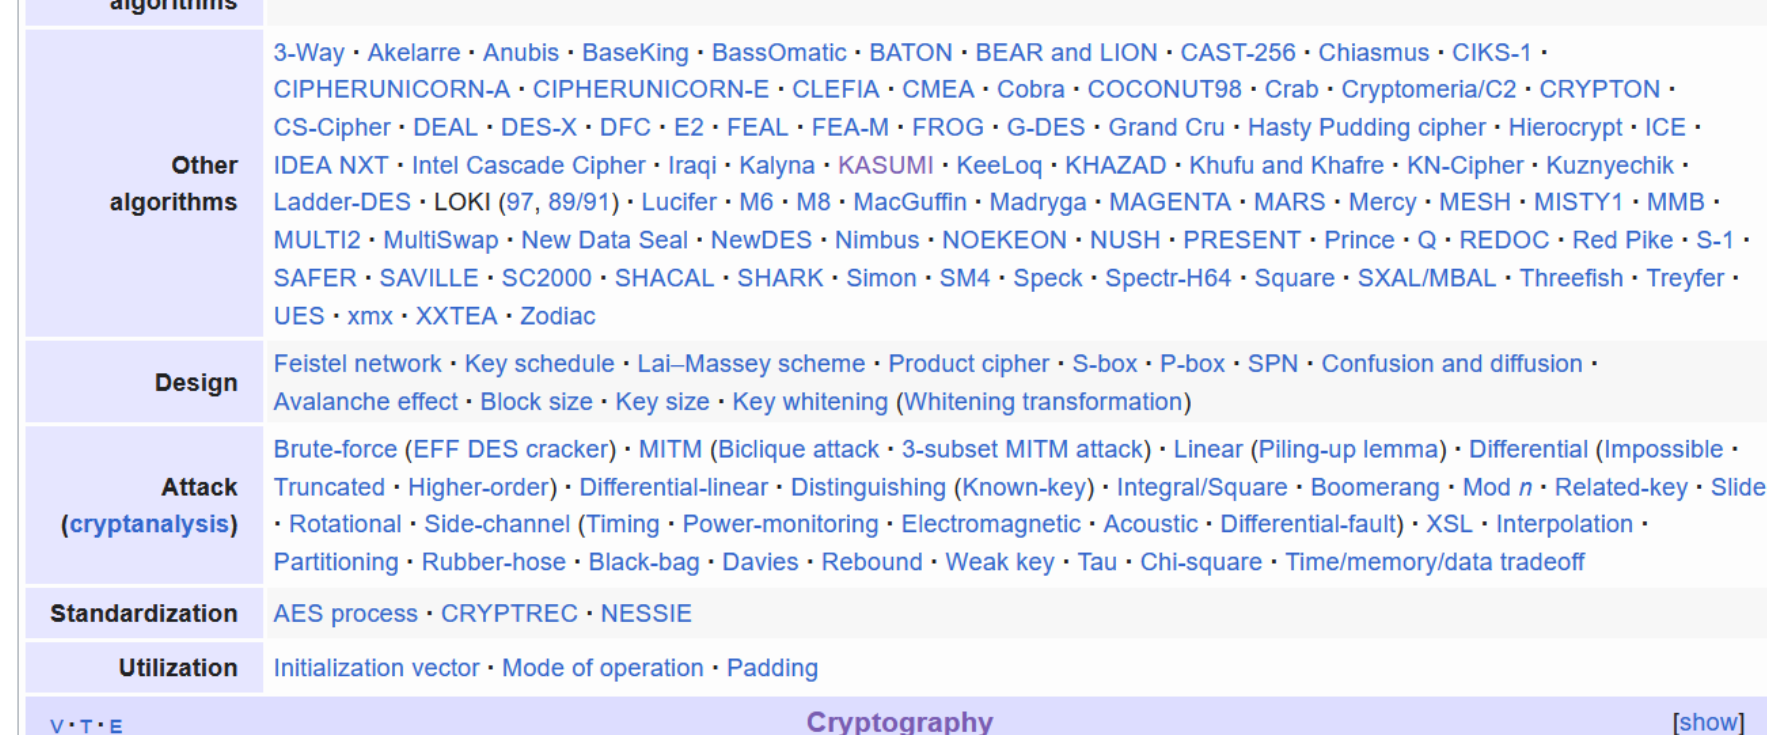
\includegraphics[width=193.20mm,height=201.96mm]{../../images/llm/page_008_img_01.png}%
\end{textblock*}

\end{document}
